\begin{frame}{Programa}
	\begin{block}{}
		\begin{itemize}
			\item Interface desenvolvida usando o ambiente \textit{GUIDE} do MATLAB.
			\vspace{1mm}
			\item Métodos de minimização vetorial feitos na forma de funções.
		\end{itemize}
		\vspace{-3mm}
		\begin{figure}[H]
			\begin{center}
				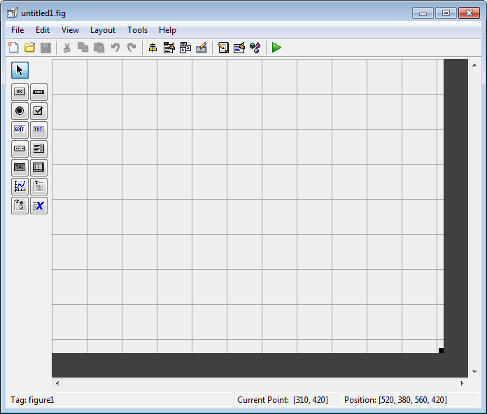
\includegraphics[width=5cm]{GUIDE}   
				\vspace{-0.15cm}
				\caption{Ambiente de desenvolvimento de interface gráfica}
				\label{fig:GUIDE}
			\end{center}
		\end{figure}
		
	\end{block}
\end{frame}
\begin{frame}{}
	\vspace{0mm}
	\hspace{4mm}
	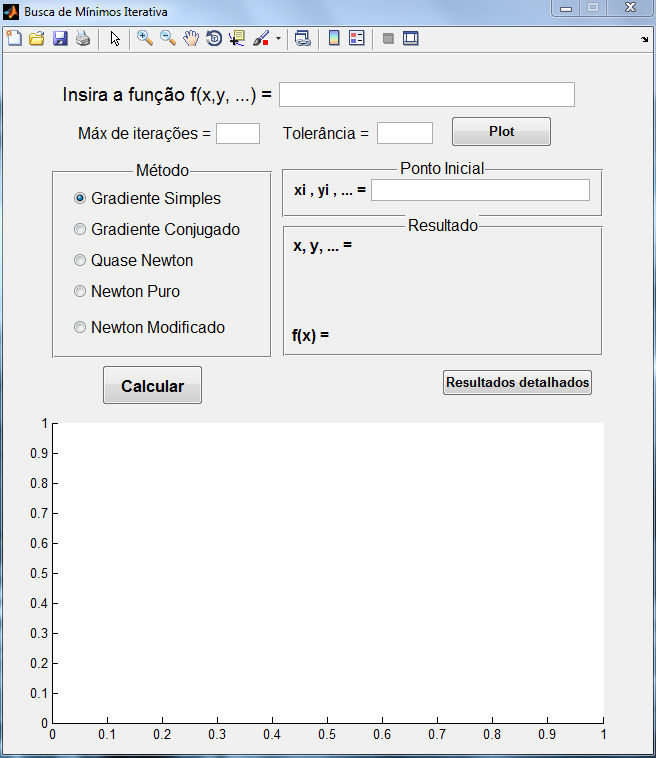
\includegraphics[scale=0.55]{GUI}
\end{frame}